\documentclass{sig-alternate}

\begin{document}
%
% --- Author Metadata here ---
\conferenceinfo{18-697}{Fall '14 Pittsburgh, PA USA}
\CopyrightYear{2014}
% --- End of Author Metadata ---

\title{Clustering for Controlling Stochastic Optimization using Feedback}
\subtitle{Applied to Newspaper Article Title Category Prediction}

\numberofauthors{2} 
\author{
\alignauthor
Kevin Brennan\\
       \affaddr{Carnegie Mellon University}\\
       \affaddr{5000 Forbes Avenue}\\
       \affaddr{Pittsburgh, PA}\\
       \email{kbrennan@andrew.cmu.edu}
% 2nd. author
\alignauthor
Gavriel Adler\\
       \affaddr{Carnegie Mellon University}\\
       \affaddr{5000 Forbes Avenue}\\
       \affaddr{Pittsburgh, PA}\\
       \email{gya@andrew.cmu.edu}\\
}


\maketitle
\begin{abstract}
In optimizing feature sets for classification, there are often multiple local optima when using tools such as genetic algorithms. In order to reduce complexity and computational cost, it is often desirable to deal with only a fixed number of solutions. One method for refining the solution set is niching through generalized crowding.\\
\indent In this paper, we explore using a genetic algorithm for creating optimized feature sets for classification problems. Through several trials of a genetic algorithm, we create a solution space of locally optimal feature sets. Using generalized crowding with K Nearest Neighbor clustering, we refine the solution space into a set of niches. Based on the difference between a desired number of niches and the returned value, we implement a feedback controller for the exploration/exploitation of the genetic algorithm. By tuning this parameter, we adjust the range of the solution space through several trials till it converges to a desired number of niches. After testing on classifying newspaper titles, the algorithm did not show the controller to be effective in converging the solution space to a desired number of niches. Control over the exploration/exploitation parameter did not have sufficient power to augment the number of niches.
\end{abstract}

\terms{Classification, Feedback, Stochastic Optimization}

\keywords{Controlled Clustering, Naive Bayes, KMeans, Title Category Classification}

\section{Introduction}
The problem of optimizing feature sets for use in classification is often multi-modal. Often there are variable number of local optima each with unique characteristics. Although multiple solutions often give a better representation of the solution space for a given optimization, having a variable number of solutions can drastically increase the complexity and cost of a given algorithm.\\
\indent One method for creating a fixed size solution set is through generalized crowding. Crowding groups solutions based on a given fitness function into a set of niches\cite{ole:feedback}. Using a scaling factor, generalized crowding controls the range of solutions  with respect to the given fitness function. In the case of evolutionary algorithms such as genetic algorithms, the scaling factor controls the exploration/exploitation parameter used in determining survival between generations. Control of the scaling factor therefore also controls the number of niches within a given solution space\cite{ole:feedback}.\\
\indent In this paper, we detail using genetic algorithm to optimize feature sets for classifying newspaper titles into topics. For classification, each feature set is a set of bit-strings. Through several trials of a genetic algorithm, we create a set of locally optimized feature sets. With K nearest neighbor, we implement generalized crowding in order to cluster the solution set into a set of niches. We apply a feedback controller on the error between the desired number of niches and this returned number. In this paper, we consider the use a full PID controller in order to expand upon past research in this area. Using derivative and integral gains allows for greater control of the rate of convergence, overshoot, and steady state error when refining the number of  niches. Further information on the implementation of our algorithm is provided in the Methods section of our paper.  

\section{Related Research}
\subsection{Feature Selection}
\cite{feature:feedback}

\subsection{Generalized Crowding}

\subsection{Feedback Controller}

\section{Method}
\begin{figure*}[t]
\centering
\fbox{
  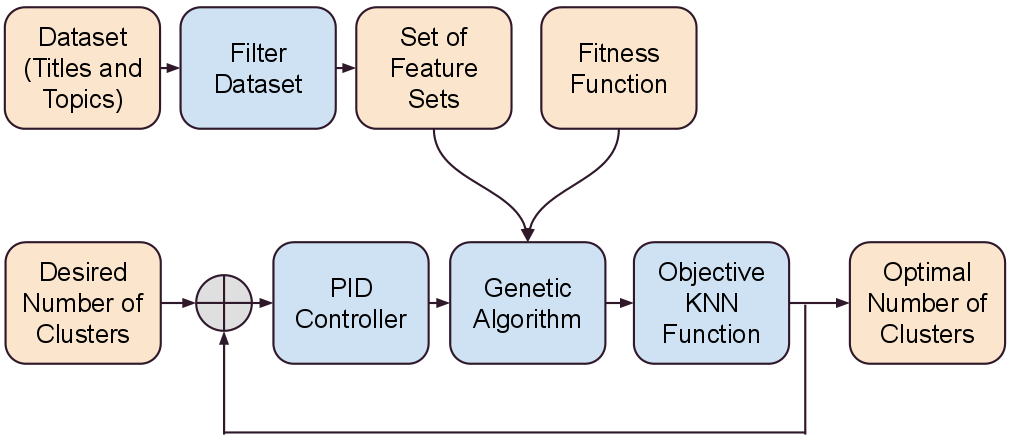
\includegraphics[width=0.8\textwidth]{pipeline.png}}
\caption{The Algorithm Pipeline}
\label{fig:pipeline}
\end{figure*}
\subsection{Pipeline Overview}
Our pipeline, as seen in Figure~\ref{fig:pipeline}, consists of a few independent pieces put together in a control loop. To initialize the pipeline, we first separated the titles into a training and a testing set. We then made a list of words that appear in the titles of the training set and filtered the data set into our feature sets, or sets of bags of words from that list. In the control loop, we get our error value from the difference between the optimal number of clusters returned by the objective K-Means function and the desired number of clusters. The error and the PID controller created a $\phi$ term representing exploration vs. exploitation. We generated sets of bags of words from the training set list and passed each into the genetic algorithm along with the $\phi$ term, and each returned a locally optimal bag of words. These optimal bags were clustered to find the optimal number of clusters, and the loop restarts. Each section of the algorithm is discussed in detail below.

\subsection{Genetic Algorithm}
\begin{figure}[t]
\centering
\fbox{\rule{0pt}{2in}
  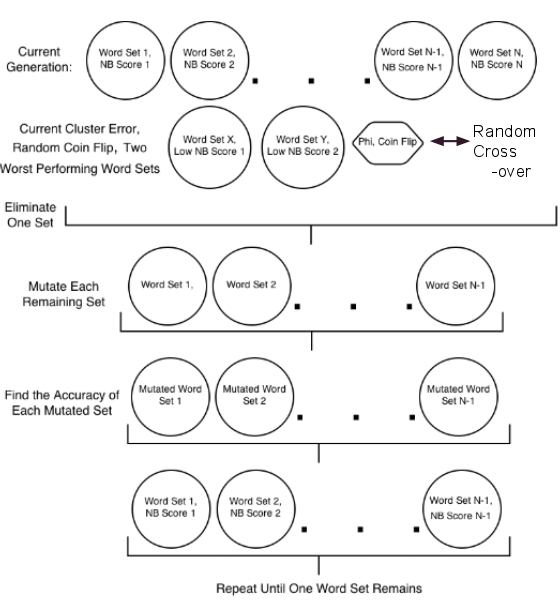
\includegraphics[width=0.45\textwidth]{genetic_algo.png}}
\caption{The flow of one iteration of the genetic algorithm}
\label{fig:genetic_algo}
\end{figure}
Our genetic algorithm operated on a set of bags of words, and converged to a single locally optimal bag of words. At each round of the genetic algorithm, the Naive Bayes score on the testing set was calculated for each bag of words. The lowest two scores competed for survival, and the victor was based on both the $\phi$ exploration/exploitation term and a random coin flip. After one bag was killed, each remaining bag was mutated and additional randomized cross-over between trials was added in to further diversity. Our solution set was created by running several trials of the genetic algorithm on many randomly generated sets of bags of words.\\
\indent In the mutation step, the algorithm attempted to replace each word in the bag of words with a new word taken from the titles in the training set. If the Naive Bayes score of the bag of words with the new word was higher than it was with the old word, the new word replaced the old word, otherwise the new word was discarded.\\
\indent This process of testing with Naive Bayes continues till only a single bag of words is left. We add this bag of words to our solution set, and after all the trials of the genetic algorithm are finished we have a set locally optimal solutions. This solution set is then passed onto the clustering algorithm.

\subsection{Clustering Algorithm}
Our clustering algorithm is based on the Objective K Nearest Neighbor function. The objective function works by running K-Means with a variable number of nodes used for clustering. For each element of the solution set created by the genetic algorithm trials, we calculate the number of true positives, false positives, true negatives, and false negative. A true positive or true negative represents the correct classification of a title, and conversely a false positive or false negative represents a failure to do so. This representation is possible because we are separating the titles into only two classes. We used these statistics, instead of other distance metrics such as the Hamming distance as used in previous research\cite{ole:feedback}, in order to cluster the solutions by characteristics. For instance, to have on group of solutions with minimal false positive or another with minimal false negatives.\\
\indent Based on these statistics, we calculate a distance to each node based on the Euclidean distance metric. For K-Means, we group each element to the closest node, and re-calculate a mean node for each grouping. K-Means continues to iterate until the mean nodes remain constant between iterations. Once K-Means finishes iterating, we calculate the distance of each element to its group's mean node. The sum of these distances is our error for that given number of nodes.\\
\indent Based on the error for each number of nodes, we find the change in the error with respect to the change in the number of nodes. This change is the first derivative for our error. Next, we find the change in the first derivative with respect to the change in the number of nodes. This change is the second derivative for our error. Based on the maximum second derivative, we calculate the elbow point for the error versus number of nodes. For our feedback loop, the elbow point returned by our clustering algorithm represents the optimal number of nodes, or local optima, to use.

\subsection{Feedback Controller}
For controlling the exploration/exploitation term for the genetic algorithm, we use a PID controller. The set point for the controller is the desired number of clusters after crowding. The error is the difference between the set point and the returned number of clusters from the clustering algorithm. Based on this error, we calculate the change in the exploration/exploitation term for the next iteration of the feedback loop. The change is determined by calculating the change in error between iterations of the feedback loop, which is our derivative term, and the sum of all past errors, which is our integral term. By multiplying these terms and the error by set gains, we calculate the new exploration/exploitation term. The goal of implementing a full PID controller is to improve upon the efficiency of the entire pipeline by reducing the number of iterations till convergence to the desired number of clusters. The derivative term should improve the responsiveness of the controller while the integral term should ensure that the limit of the error goes to zero in time.

\subsection{Implementation}
We implemented our pipeline using Python's PANDAS module. Python, a scripting language, is easy to work with and develop quickly which was important given the project had to be finished within a semester. PANDAS is built on top of Python's NumPy library, which is strictly typed and invokes C calls, significantly speeding up the slow execution of Python. Lastly, we implemented clustering using Python's scikit-learn library, a machine learning library. Scikit-learn is also built in NumPy, making passing data between the two libraries very simple. In the end we were able to run our pipeline very efficiently, with each iteration of the feedback loop taking on the order of seconds instead of minutes. This speed allowed us to try many different runs of various combinations of parameters and analyze the results.

\section{Results}
In the end we found this approach did not fare well and the results converged to a single cluster very quickly, and therefore would recommend not using our process but Hamming

\section{Conclusion and Future Work}
This paper details the use of genetic algorithm, clustering, and feedback control in order to fixed-size optimized feature sets for classification. A PID controller adjusts the parameters of the genetic algorithm in order to control the range of the solution space. Clustering groups the solution space into a set of niches. This set of niches determines the error for the control loop in the next iteration of the feedback loop. This paper explores the use of derivative and integral terms in order to increase the responsiveness of the controller. In addition, it explore the use of different distance metrics used for clustering in order to investigate the characteristics of each of the solution space's niches. Although the results did not yield great success in controlling the solution space, the work detailed leaves several areas for further investigation and experimentation.\\
\indent For future work, we would experiment with other distance metrics for clustering. As mentioned in the results section, the classification results proved to be similar to create substantial differences in clustering. This similarity caused the solution set to sometimes converge to a single cluster, which impede the feedback controller.\\
\indent Another area for future work would be the creation of classification rules in the genetic algorithm. In our current algorithm, we relies solely on Naive Bayes as the classifier for a given feature. By expanding upon Naive Bayes, we could implement a decision tree based on the Naive Bayes results for each element of a given feature set. This expansion should improve the classification scores of the feature set as it considers combinations of words in a title rather just each word by itself.

\bibliography{sigproc.bib}
\bibliographystyle{plain}

\end{document}
